\begin{vdmpp}
class TestPetriNet is subclass of MyTestCase

operations
  /**
   * Requirements: R1, R2.3, R2.4, R3, R4, R5
   */
(*@
\label{testElevator1Example:4}
@*)
(*@
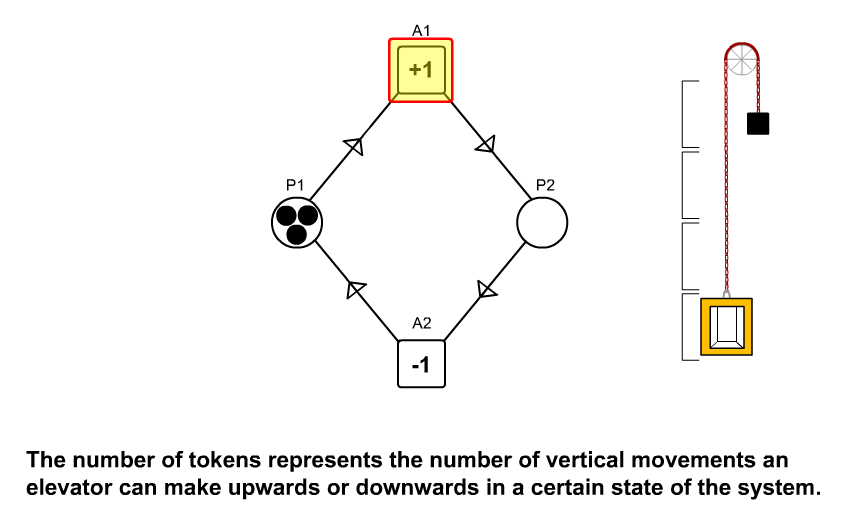
\includegraphics[width=5cm]{specification/elevator1.png}
@*)
  public testElevator1Example: () ==> ()
  testElevator1Example() == (
    /* http://www.informatik.uni-hamburg.de/TGI/PetriNets/introductions/aalst/elevator1.swf */
    IO`println("\t\t test elevator 1");
    let p1 = new Place("P1", 3),
     p2 = new Place("P2", 3),
     a1i = new WeightedInputArc(p1, 1),
     a1o = new WeightedOutputArc(p2, 1),
     a2i = new WeightedInputArc(p2, 1),
     a2o = new WeightedOutputArc(p1, 1),
     t1 = new Transition("+1", { a1i }, { a1o }),
     t2 = new Transition("-1", { a2i }, { a2o }),

     places = { p1, p2 },
     arcs = { a1i, a1o, a2i, a2o },
     marking = { p1 |-> 3, p2 |-> 0 },
     transitions = { t1, t2 },

     petriNet = new PetriNet(places, p1, {}, arcs, marking, transitions) in (

      assertEqual({ p1 |-> 3, p2 |-> 0 }, petriNet.marking);

      /* Test reachability of the markings before step execution */
      assertTrue(petriNet.isReachable({ p1 |-> 2, p2 |-> 1 }));
      assertTrue(petriNet.isReachable({ p1 |-> 1, p2 |-> 2 }));
      assertTrue(petriNet.isReachable({ p1 |-> 0, p2 |-> 3 }));
      assertTrue(not petriNet.isReachable({ p1 |-> 4, p2 |-> 5 }));

      assertEqual({}, petriNet.getAllSequences(
        { p1 |-> 3, p2 |-> 0 },{ p1 |-> 4, p2 |-> 5 })
      );
      assertEqual({[t1, t1]}, petriNet.getAllSequences(
        { p1 |-> 3, p2 |-> 0 }, { p1 |-> 1, p2 |-> 2 })
      );
      assertEqual({[t1, t1, t1]}, petriNet.getAllSequences(
        { p1 |-> 3, p2 |-> 0 }, { p1 |-> 0, p2 |-> 3 })
      );

      /* Test stepwise execution of the petri net */
      petriNet.executeStep(t1);
      assertEqual({ p1 |-> 2, p2 |-> 1 }, petriNet.marking);

      petriNet.executeStep(t1);
      assertEqual({ p1 |-> 1, p2 |-> 2 }, petriNet.marking);

      petriNet.executeStep(t1);
      assertEqual({ p1 |-> 0, p2 |-> 3 }, petriNet.marking);

      petriNet.executeStep(t2);
      assertEqual({ p1 |-> 1, p2 |-> 2 }, petriNet.marking);

      petriNet.executeStep(t1);
      assertEqual({ p1 |-> 0, p2 |-> 3 }, petriNet.marking);
    );
  );

  /**
   * Requirements: R1, R2.3, R2.4, R3, R4, R5
   */
(*@
\label{testElevator2Example:60}
@*)
(*@
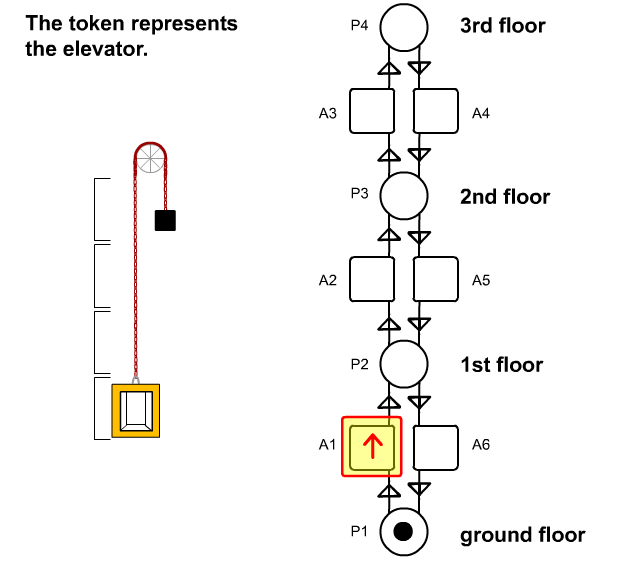
\includegraphics[width=5cm]{specification/elevator2.png}
@*)
  public testElevator2Example: () ==> ()
  testElevator2Example() == (
    /* http://www.informatik.uni-hamburg.de/TGI/PetriNets/introductions/aalst/elevator2.swf */
    IO`println("\t\t test elevator 2");
    let p1 = new Place("ground floor", 1),
     p2 = new Place("1st floor", 1),
     p3 = new Place("2nd floor", 1),
     p4 = new Place("3rd floor", 1),
     a1i = new WeightedInputArc(p1, 1),
     a1o = new WeightedOutputArc(p2, 1),
     a2i = new WeightedInputArc(p2, 1),
     a2o = new WeightedOutputArc( p3, 1),
     a3i = new WeightedInputArc(p3, 1),
     a3o = new WeightedOutputArc(p4, 1),
     a4i = new WeightedInputArc(p4, 1),
     a4o = new WeightedOutputArc(p3, 1),
     a5i = new WeightedInputArc(p3, 1),
     a5o = new WeightedOutputArc(p2, 1),
     a6i = new WeightedInputArc(p2, 1),
     a6o = new WeightedOutputArc(p1, 1),
     t1 = new Transition("A1", { a1i }, { a1o }),
     t2 = new Transition("A2", { a2i }, { a2o }),
     t3 = new Transition("A3", { a3i }, { a3o }),
     t4 = new Transition("A4", { a4i }, { a4o }),
     t5 = new Transition("A5", { a5i }, { a5o }),
     t6 = new Transition("A6", { a6i }, { a6o }),

     places = { p1, p2, p3, p4 },
     arcs = { a1i, a1o, a2i, a2o, a3i, a3o, a4i, a4o, a5i, a5o, a6i, a6o },
     marking = { p1 |-> 1, p2 |-> 0, p3 |-> 0, p4 |-> 0 },
     transitions = { t1, t2, t3, t4, t5, t6 },

     petriNet = new PetriNet(places, p1, {}, arcs, marking, transitions) in (

      /* Test reachability before stepwise execution */
      assertTrue(petriNet.isReachable({ p1 |-> 1, p2 |-> 0, p3 |-> 0, p4 |-> 0 }));
      assertTrue(petriNet.isReachable({ p1 |-> 0, p2 |-> 1, p3 |-> 0, p4 |-> 0 }));
      assertTrue(petriNet.isReachable({ p1 |-> 0, p2 |-> 1, p3 |-> 0, p4 |-> 0 }));

      assertEqual({ p1 |-> 1, p2 |-> 0, p3 |-> 0, p4 |-> 0 }, petriNet.marking);

      /* Test stepwise execution of the Petri net */
      petriNet.executeStep(t1); /* valid */
      assertEqual({ p1 |-> 0, p2 |-> 1, p3 |-> 0, p4 |-> 0 }, petriNet.marking);

      petriNet.executeStep(t2); /* valid */
      assertEqual({ p1 |-> 0, p2 |-> 0, p3 |-> 1, p4 |-> 0 }, petriNet.marking);

      petriNet.executeStep(t5); /* valid */
      assertEqual({ p1 |-> 0, p2 |-> 1, p3 |-> 0, p4 |-> 0 }, petriNet.marking);

      let previousMarking = petriNet.marking in (
        petriNet.executeStep(t1); /* not valid, no marking change */
        assertEqual(previousMarking, petriNet.marking);
      )
    );
  );

  /**
   * Requirements: R1, R2.3, R2.4, R3, R4, R5
   */
(*@
\label{testElevator3Example:118}
@*)
(*@
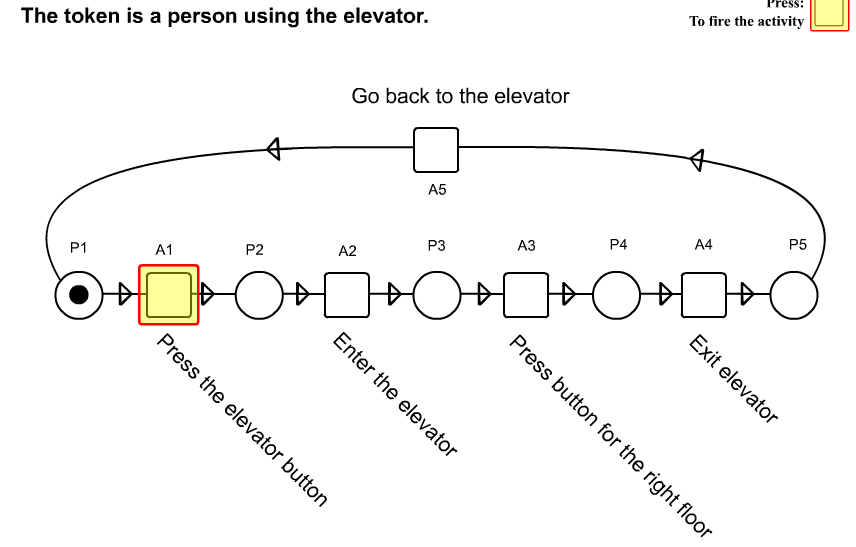
\includegraphics[width=5cm]{specification/elevator3.png}
@*)
  public testElevator3Example: () ==> ()
  testElevator3Example() == (
    /* http://www.informatik.uni-hamburg.de/TGI/PetriNets/introductions/aalst/elevator3.swf */
    IO`println("\t\t test elevator 3");
    let p1 = new Place("p1", 1),
     p2 = new Place("p2", 1),
     p3 = new Place("p3", 1),
     p4 = new Place("p4", 1),
     p5 = new Place("p5", 1),
     a1i = new WeightedInputArc(p1,  1),
     a1o = new WeightedOutputArc(p2, 1),
     a2i = new WeightedInputArc(p2, 1),
     a2o = new WeightedOutputArc(p3, 1),
     a3i = new WeightedInputArc(p3, 1),
     a3o = new WeightedOutputArc(p4, 1),
     a4i = new WeightedInputArc(p4, 1),
     a4o = new WeightedOutputArc(p5, 1),
     a5i = new WeightedInputArc(p5, 1),
     a5o = new WeightedOutputArc(p1, 1),
     t1 = new Transition("A1 - Press the elevator button", { a1i }, { a1o }),
     t2 = new Transition("A2 - Enter the elevator", { a2i }, { a2o }),
     t3 = new Transition("A3 - Press button for the right floor", { a3i }, { a3o }),
     t4 = new Transition("A4 - Exit elevator", { a4i }, { a4o }),
     t5 = new Transition("A5 - Go back to the elevator", { a5i }, { a5o }),

     places = { p1, p2, p3, p4, p5 },
     arcs = { a1i, a1o, a2i, a2o, a3i, a3o, a4i, a4o, a5i, a5o },
     marking = { p1 |-> 1, p2 |-> 0, p3 |-> 0, p4 |-> 0, p5 |-> 0 },
     transitions = { t1, t2, t3, t4, t5 },

     petriNet = new PetriNet(places, p1, {}, arcs, marking, transitions) in (

      /* Test reachability before stepwise execution */
      assertTrue(petriNet.isReachable({ p1 |-> 1, p2 |-> 0, p3 |-> 0, p4 |-> 0, p5 |-> 0 }));
      assertTrue(petriNet.isReachable({ p1 |-> 0, p2 |-> 1, p3 |-> 0, p4 |-> 0, p5 |-> 0 }));
      assertTrue(petriNet.isReachable({ p1 |-> 0, p2 |-> 0, p3 |-> 1, p4 |-> 0, p5 |-> 0 }));
      assertTrue(petriNet.isReachable({ p1 |-> 0, p2 |-> 0, p3 |-> 0, p4 |-> 1, p5 |-> 0 }));
      assertTrue(petriNet.isReachable({ p1 |-> 0, p2 |-> 0, p3 |-> 0, p4 |-> 0, p5 |-> 1 }));

      assertEqual({ p1 |-> 1, p2 |-> 0, p3 |-> 0, p4 |-> 0, p5 |-> 0 }, petriNet.marking);

      /* Test stepwise execution of the petri net */
      petriNet.executeStep(t1); /* valid */
      assertEqual({ p1 |-> 0, p2 |-> 1, p3 |-> 0, p4 |-> 0, p5 |-> 0 }, petriNet.marking);

      petriNet.executeStep(t2); /* valid */
      assertEqual({ p1 |-> 0, p2 |-> 0, p3 |-> 1, p4 |-> 0, p5 |-> 0 }, petriNet.marking);

      petriNet.executeStep(t3); /* valid */
      assertEqual({ p1 |-> 0, p2 |-> 0, p3 |-> 0, p4 |-> 1, p5 |-> 0 }, petriNet.marking);

      petriNet.executeStep(t4); /* valid */
      assertEqual({ p1 |-> 0, p2 |-> 0, p3 |-> 0, p4 |-> 0, p5 |-> 1 }, petriNet.marking);

      petriNet.executeStep(t5); /* valid */
      assertEqual({ p1 |-> 1, p2 |-> 0, p3 |-> 0, p4 |-> 0, p5 |-> 0 }, petriNet.marking);

    );
  );

  /**
   * Requirements: R1, R2.2, R2.3, R2.4, R3, R4
   */
(*@
\label{testSimpleInhibitorArc:178}
@*)
(*@
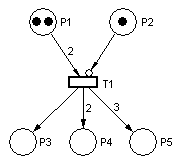
\includegraphics[width=5cm]{specification/simpleinhibitorarc.png}
@*)
  public testSimpleInhibitorArc: () ==> ()
  testSimpleInhibitorArc() == (
    /* http://www.techfak.uni-bielefeld.de/~mchen/BioPNML/Intro/pnfaq_files/image005.gif */
    IO`println("\t\t test simple inhibitor arc");
    let p1 = new Place("P1", 2),
     p2 = new Place("P2", 1),
     p3 = new Place("P3", 1),
     p4 = new Place("P4", 3),
     p5 = new Place("P5", 4),
     ia1 = new WeightedInputArc(p1,  2),
     ia2 = new InhibitorArc(p2),
     oa1 = new WeightedOutputArc(p3, 1),
     oa2 = new WeightedOutputArc(p4, 2),
     oa3 = new WeightedOutputArc(p5, 3),
     t1 = new Transition("T1", { ia1, ia2 }, { oa1, oa2, oa3 }),

     places = { p1, p2, p3, p4, p5 },
     arcs = { ia1, ia2, oa1, oa2, oa3 },
     marking1 = { p1 |-> 2, p2 |-> 1, p3 |-> 0, p4 |-> 0, p5 |-> 0 },
     marking2 = { p1 |-> 2, p2 |-> 0, p3 |-> 0, p4 |-> 0, p5 |-> 0 },
     transitions = { t1 },

     petriNet1 = new PetriNet(places, p1, {}, arcs, marking1, transitions),
     petriNet2 = new PetriNet(places, p1, {}, arcs, marking2, transitions) in (

      assertEqual({ p1 |-> 2, p2 |-> 1, p3 |-> 0, p4 |-> 0, p5 |-> 0 }, petriNet1.marking);
      assertEqual({ p1 |-> 2, p2 |-> 0, p3 |-> 0, p4 |-> 0, p5 |-> 0 }, petriNet2.marking);

      assertTrue(not petriNet1.isReachable(
        { p1 |-> 0, p2 |-> 0, p3 |-> 1, p4 |-> 2, p5 |-> 3 })
      );
      assertTrue( petriNet2.isReachable(
        { p1 |-> 0, p2 |-> 0, p3 |-> 1, p4 |-> 2, p5 |-> 3 })
      );

      petriNet1.executeStep(t1); /* should not trigger */
      petriNet2.executeStep(t1); /* should trigger */

      assertEqual({ p1 |-> 2, p2 |-> 1, p3 |-> 0, p4 |-> 0, p5 |-> 0 }, petriNet1.marking);
      assertEqual({ p1 |-> 0, p2 |-> 0, p3 |-> 1, p4 |-> 2, p5 |-> 3 }, petriNet2.marking);
    );
  );

  /**
   * Requirements: R1, R2.1, R2.3, R2.4, R3, R4
   */
(*@
\label{testSimpleResetArc:221}
@*)
(*@
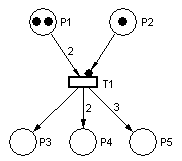
\includegraphics[width=5cm]{specification/simpleresetarc.png}
@*)
  public testSimpleResetArc: () ==> ()
  testSimpleResetArc() == (
    /* http://www.techfak.uni-bielefeld.de/~mchen/BioPNML/Intro/pnfaq_files/image003.gif (mod.) */
    IO`println("\t\t test simple reset arc");
    let p1 = new Place("P1", 2),
     p2 = new Place("P2", 1),
     p3 = new Place("P3", 1),
     p4 = new Place("P4", 3),
     p5 = new Place("P5", 4),
     ia1 = new WeightedInputArc(p1,  2),
     ia2 = new ResetArc(p2),
     oa1 = new WeightedOutputArc(p3, 1),
     oa2 = new WeightedOutputArc(p4, 2),
     oa3 = new WeightedOutputArc(p5, 3),
     t1 = new Transition("T1", { ia1, ia2 }, { oa1, oa2, oa3 }),

     places = { p1, p2, p3, p4, p5 },
     arcs = { ia1, ia2, oa1, oa2, oa3 },
     marking1 = { p1 |-> 2, p2 |-> 5, p3 |-> 0, p4 |-> 0, p5 |-> 0 },
     marking2 = { p1 |-> 2, p2 |-> 0, p3 |-> 0, p4 |-> 0, p5 |-> 0 },
     transitions = { t1 },

     petriNet1 = new PetriNet(places, p1, {}, arcs, marking1, transitions),
     petriNet2 = new PetriNet(places, p1, {}, arcs, marking2, transitions) in (

      assertEqual({ p1 |-> 2, p2 |-> 5, p3 |-> 0, p4 |-> 0, p5 |-> 0 }, petriNet1.marking);
      assertEqual({ p1 |-> 2, p2 |-> 0, p3 |-> 0, p4 |-> 0, p5 |-> 0 }, petriNet2.marking);

      assertTrue(petriNet1.isReachable({ p1 |-> 0, p2 |-> 0, p3 |-> 1, p4 |-> 2, p5 |-> 3 }));
      assertTrue(petriNet2.isReachable({ p1 |-> 0, p2 |-> 0, p3 |-> 1, p4 |-> 2, p5 |-> 3 }));

      petriNet1.executeStep(t1); /* should trigger */
      petriNet2.executeStep(t1); /* should trigger */

      assertEqual({ p1 |-> 0, p2 |-> 0, p3 |-> 1, p4 |-> 2, p5 |-> 3 }, petriNet1.marking);
      assertEqual({ p1 |-> 0, p2 |-> 0, p3 |-> 1, p4 |-> 2, p5 |-> 3 }, petriNet2.marking);
    );
  );

  /**
   * Requirements: R1, R2.3, R2.4, R3, R4
   */
(*@
\label{testSimpleCapacityArc:260}
@*)
(*@
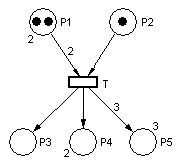
\includegraphics[width=5cm]{specification/simplecapacityarc.png}
@*)
  public testSimpleCapacityArc: () ==> ()
  testSimpleCapacityArc() == (
    /* http://www.techfak.uni-bielefeld.de/~mchen/BioPNML/Intro/pnfaq_files/image003.gif (mod.) */
    IO`println("\t\t test simple capacity arc");
    let p1 = new Place("P1", 2),
     p2 = new Place("P2", 1),
     p3 = new Place("P3", 1),
     p4 = new Place("P4", 2),
     p5 = new Place("P5", 3),
     ia1 = new WeightedInputArc(p1,  2),
     ia2 = new WeightedInputArc(p2,  1),
     oa1 = new WeightedOutputArc(p3, 1),
     oa2 = new WeightedOutputArc(p4, 2),
     oa3 = new WeightedOutputArc(p5, 3),
     t1 = new Transition("T1", { ia1, ia2 }, { oa1, oa2, oa3 }),

     places = { p1, p2, p3, p4, p5 },
     arcs = { ia1, ia2, oa1, oa2, oa3 },
     marking1 = { p1 |-> 2, p2 |-> 1, p3 |-> 0, p4 |-> 0, p5 |-> 3 },
     marking2 = { p1 |-> 2, p2 |-> 1, p3 |-> 0, p4 |-> 0, p5 |-> 0 },
     transitions = { t1 },

     petriNet1 = new PetriNet(places, p1, {}, arcs, marking1, transitions),
     petriNet2 = new PetriNet(places, p1, {}, arcs, marking2, transitions) in (

      assertEqual({ p1 |-> 2, p2 |-> 1, p3 |-> 0, p4 |-> 0, p5 |-> 3 }, petriNet1.marking);
      assertEqual({ p1 |-> 2, p2 |-> 1, p3 |-> 0, p4 |-> 0, p5 |-> 0 }, petriNet2.marking);

      assertTrue(not petriNet1.isReachable(
        { p1 |-> 0, p2 |-> 0, p3 |-> 1, p4 |-> 2, p5 |-> 3 })
      );
      assertTrue(petriNet2.isReachable(
        { p1 |-> 0, p2 |-> 0, p3 |-> 1, p4 |-> 2, p5 |-> 3 })
      );

      petriNet1.executeStep(t1); /* should not trigger */
      petriNet2.executeStep(t1); /* should trigger */

      assertEqual({ p1 |-> 2, p2 |-> 1, p3 |-> 0, p4 |-> 0, p5 |-> 3 }, petriNet1.marking);
      assertEqual({ p1 |-> 0, p2 |-> 0, p3 |-> 1, p4 |-> 2, p5 |-> 3 }, petriNet2.marking);
    );
  );

  /* Entry point that runs all tests with valid inputs */
(*@
\label{testAll:304}
@*)
  public testAll: () ==> ()
  testAll() == (
    IO`println("\t petrinet tests");
    testElevator1Example();
    testElevator2Example();
    testElevator3Example();
    testSimpleInhibitorArc();
    testSimpleResetArc();
    testSimpleCapacityArc();
  );

end TestPetriNet
\end{vdmpp}
\bigskip
\begin{longtable}{|l|r|r|r|}
\hline
Function or operation & Line & Coverage & Calls \\
\hline
\hline
\hyperref[testAll:304]{testAll} & 304&100.0\% & 1 \\
\hline
\hyperref[testElevator1Example:4]{testElevator1Example} & 4&100.0\% & 1 \\
\hline
\hyperref[testElevator2Example:60]{testElevator2Example} & 60&100.0\% & 1 \\
\hline
\hyperref[testElevator3Example:118]{testElevator3Example} & 118&100.0\% & 1 \\
\hline
\hyperref[testSimpleCapacityArc:260]{testSimpleCapacityArc} & 260&100.0\% & 1 \\
\hline
\hyperref[testSimpleInhibitorArc:178]{testSimpleInhibitorArc} & 178&100.0\% & 1 \\
\hline
\hyperref[testSimpleResetArc:221]{testSimpleResetArc} & 221&100.0\% & 1 \\
\hline
\hline
TestPetriNet.vdmpp & & 100.0\% & 7 \\
\hline
\end{longtable}